\chapter{State-Management Ansätze}

Bei den populären SM Lösungen folgen Redux und NgRx dem Flux-Pattern\cite{historyOfRedux}\cite{ngrxGettingStarted}, wobei Zustand und Pinia einen anderen, Framework-nahen Ansatz verfolgen.

\section{Redux}

Im Folgenden wird die Funktionsweise und die Eigenschaften von Redux näher beschrieben Die APIs von NgRx unterscheiden sich aufgrund von Bequemlichkeit, allerdings sind die Konzepte immer noch anwendbar.

Redux definiert sich durch folgenden drei Eigenschaften:
\begin{enumerate}
  \item Unveränderlichkeit (Immutability): Änderung am State sind ausschließlich über die APIs von Redux möglich.
  \item Zentralisierung des Zustandes: Der gesamte Applikationszustand lebt in einem zentralen JavaScript Objekt.
  \item Nachvollzierbarkeit (Traceability): Während der gesamten Lebensdauer der Applikation sind Änderungen am Zustand auf deren Ursprung verfolgbar.
  \item Event basiert: Es wird das Beobachter-Muster (Observer Pattern) verwendet.
\end{enumerate}

Das Verhalten des Stores wird durch \textit{actions} und \textit{reducer} definiert.
% Außerdem können optionale \textit{selectors} benutzt werden um aus bestimmten Teilen des Zustandes zu lesen.

\subsection{Actions}

Eine Aktion (Action) beschreibt eine Änderung oder Interaktion in und mit der Applikation. Beispielsweise könnte eine \textit{counter-clicked} Action versendet (dispatch) werden, wenn der Nutzer auf den \textit{Zähler erhöhen} Button drückt. Oder, wenn der Nutzer sich erfolgreich angemeldet hat, kann eine entsprechende Action versendet werden. Intern ist eine Action ein POJO.\cite{reduxStateActionReducers}

Es wird folgende Struktur für Actions empfohlen:
\begin{lstlisting}
type Action<T> = {
  type: string,
  payload: T
}
\end{lstlisting}

Das Feld \textit{type} beschreibt die Action und das optionale Feld \textit{payload} enthält weiterführende Daten.

\subsection{Reducer}

Ein Reducer übernimmt die Rolle des Beobachters und ist für die Initialisierung und Aktualisierung des Zustandes zuständig. Ein Reducer wird als eine Pure-Funtion mit zwei Parametern definiert.
Der erste Parameter ist das Zustandsobjekt und der zweite die Action. Der Rückgabewert der dieser Callback-Funcion ist das neue Zustandsobjekt. Da es sich hier um eine Pure-Funtion handelt, dürfen es hier keine Seiteneffekte stattfinden. Wie anfangserwähnt, ist der Zustand Unveränderlich, daher dürfen hier keine direkten Veränderungen des Zustandes stattfinden. Es wird lediglich ein neues Objekt zurückgegeben. Fall es keine Veränderungen stattfinden sollen, kann das ursprüngliche Objekt aus dem ersten Parameter unverändert zurückgegeben werden.\cite{reduxStateActionReducers}

Es wird folgende Struktur für Reducer empfohlen:
\begin{lstlisting}
type Reducer<S, A> = (state: S, action: A) => S
\end{lstlisting}

Beispiel reducer:

\begin{lstlisting}
function reducer(state = { user: null }, action) {
  switch (action.type) {
    case 'user-logged-in':
      return {
        ...state,
        user: {
          userId: action.payload.userId
        },
      }
    case 'user-logged-out':
      return {
        ...state,
        user: null,
      }
    default:
      return state
  }
}
\end{lstlisting}

Es wird die \textit{Spread Syntax: ...} aus ECMAScript 6 genutzt, um as ursprüngliche Zustandsobjekt zu klonen.\cite{mdnSpreadSyntax}

\subsection{Interaktion mit dem Store}

Der Store wird mit Hilfe der \textit{createStore} API erstellt. Als Parameter wird die Reducer-Function übergeben. Der Rückgabewert ist das Store-Objekt. Dieses bietet Zugang zu unteranderem \textit{dispatch} und \textit{getState} Methoden. Mit diesen kann jeweils Actions versendet und aus dem Store gelesen werden.

\begin{lstlisting}
import { createStore } from 'redux'

const store = createStore(reducer)
store.dispatch(action)
const user = store.getState().user
\end{lstlisting}

\begin{figure}[h!]
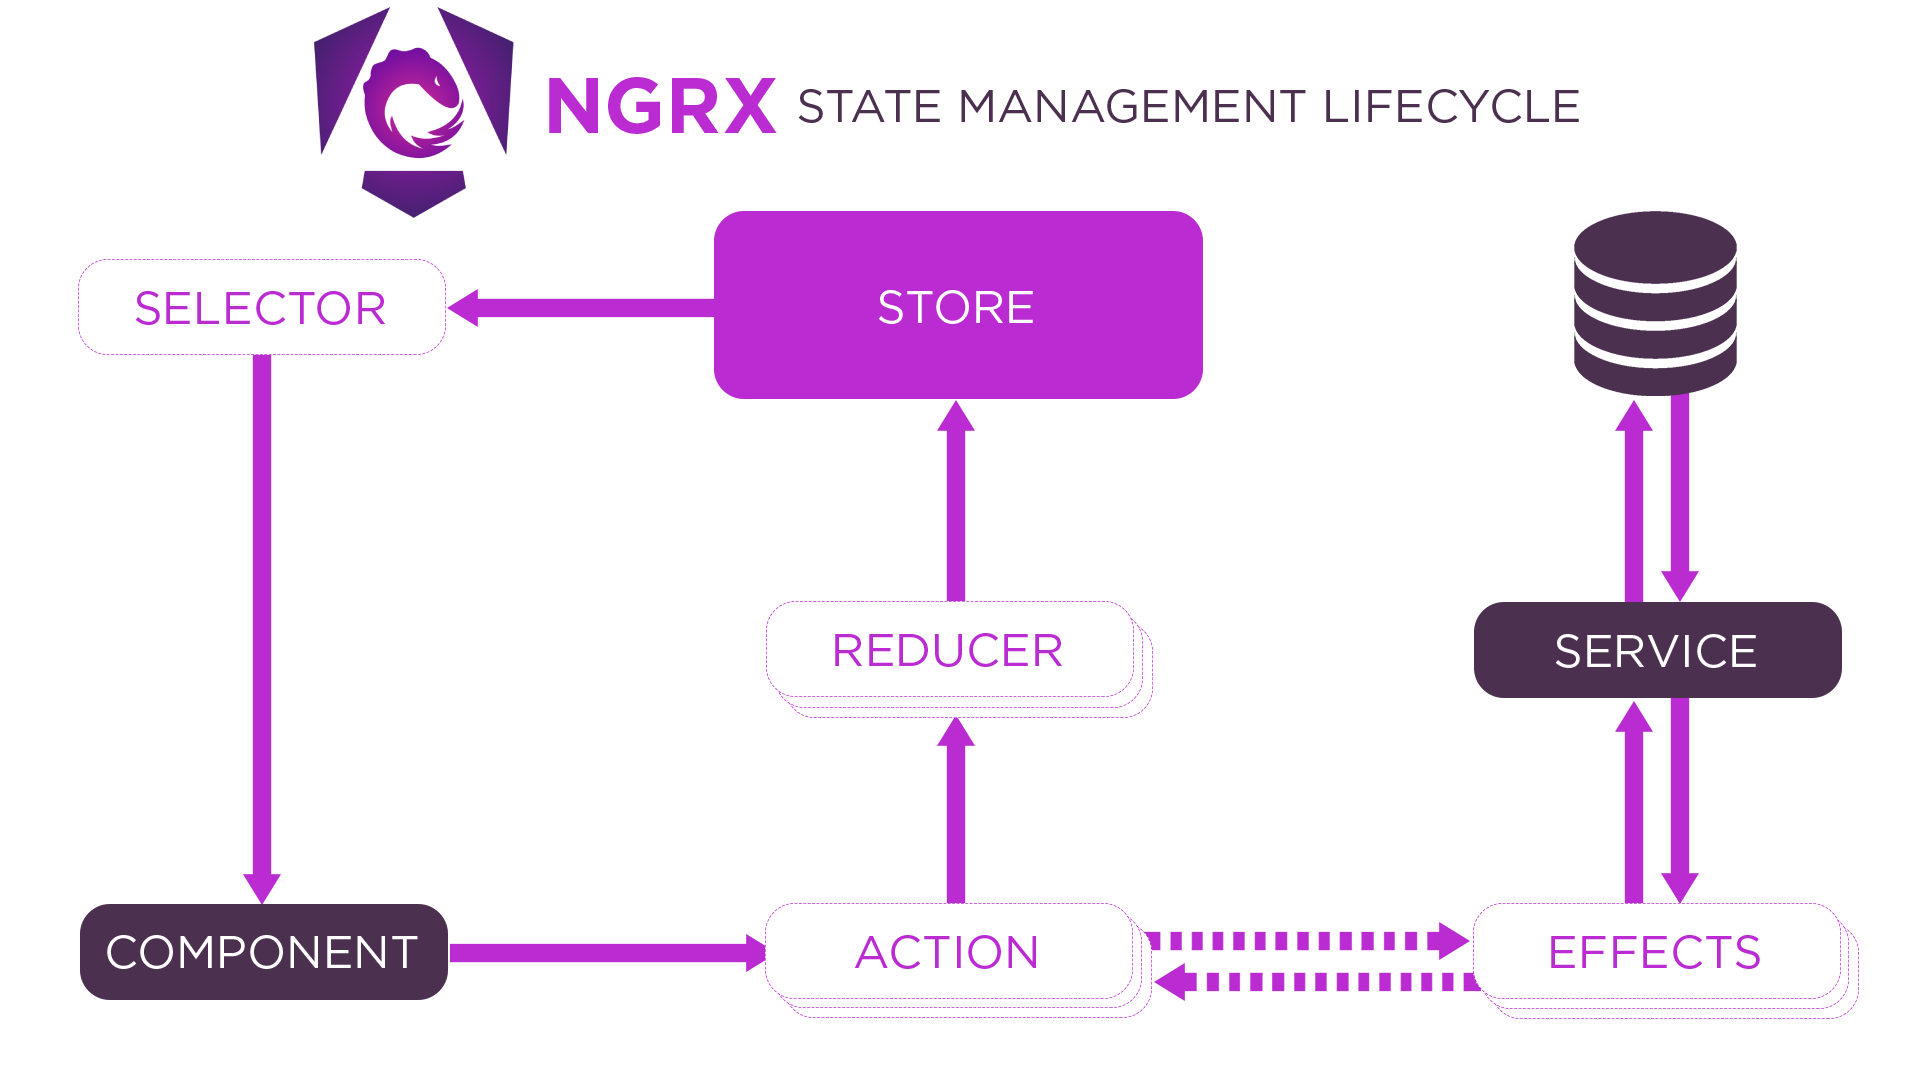
\includegraphics[width=1\textwidth]{state-management-lifecycle.png}
\caption{NgRx Datenfluss}
\end{figure}